\subsection{Advection and Hyperbolic Problems}

We will begin first with the linear advection problem as many hyperbolic problems can be rewritten in a manner similar to advection. 
\be
\ddt{f(t,x)} + v\ddx{f(t,x)} = 0,
\ee
where $v$ is some propagating speed. We will assume some initial condition $f(0,x)$ and lets assume periodic boundary conditions $f(t,0) = f(t,L)$.  The solution to this problem is trivial: $f(t,x) = g(x-vt)$ for any arbitrary function $g$.  Because such a simple analytic solution exists, these is an ideal test case to test the error of whatever method we bring to bear.

\subsubsection{Finite Difference}

The first way we will look at this is via finite difference. Lets try a very simple discretization:
\be
\frac{f^{n+1}_i - f^n_i}{\Delta t} - v\frac{f^n_{i+1} - f^n_{i-1}}{2\Delta x} = 0
\ee
This is centered differencing in space and first order differencing in time or FTCS.  For a constant $v$, we can write this as
\be
f^{n+1}_i = f^n_i - \frac{v\Delta t}{2\Delta x}\left(f^n_{i+1} - f^n_{i-1}\right) = f^n_i - \frac{\alpha_{\rm CFL}}{2}\left(f^n_{i+1} - f^n_{i-1}\right),
\ee
where $\alpha_{\rm CFL} = v\Delta t/\Delta x$ is called the Courant-Friedrichs-Levy (CFL) number.  By setting this number, we force what $\Delta t$ will be.  This is the timestep. For stability, $\alpha_{\rm CFL} < 1$ and can be much smaller than unity. This is the same statement as information does not propagate more then one cell at a time.  

We write a simple code to evolve the advection equations here.  It evolves a simple gaussian or tophat profile across a period box of length $L=1$ at a velocity of $v=1$.  The CFL number is 0.8.  We will present the code later on, but the evolution part looks like this:

\begin{lstlisting}[language=Python]
def ftcs(f, dt, dx, cfl=cfl) :
    pass
\end{lstlisting}

If we evolve this, we see that the code appears stable for a little while before it falls apart.  For the tophat profile the situation is dire immediately.  

Now the issue is the FTCS is not stable and, in fact, it is what we call unconditionally unstable, which is a bad state of affairs.  The reason for this is that information in flows moves from upstream to downstream, but the ftcs scheme above allows information to flow from downstream to upstream.  So like the future affecting the past, this is now allowed and results in the destruction of the computational universe.  

To resolve this lets define two first order spatial derivatives
\be
\frac{f^{n+1}_i - f^n_i}{\Delta t} - v\frac{f^n_{i+1} - f^n_{i}}{\Delta x} = 0 \qquad\textrm{for\ } v < 0\\
\frac{f^{n+1}_i - f^n_i}{\Delta t} - v\frac{f^n_{i} - f^n_{i-1}}{\Delta x} = 0 \qquad\textrm{for\ } v > 0 
\ee
where we pick the upwind difference, e.g., we look at which way the flow is coming.  

Lets look at the complete code now.

\lstinputlisting[language=Python]{code/advection_ftcs.py}

There are other methods to do the solutions other than upwinding.  These include Lax-Friedrichs and Lax-Wendroff, but we will move onto finite volume methods.   

Before doing so, we should discuss convergence. Convergence is the measure of how accurately a numerical method reproduces the exact solution.  In the case of ODEs, we care about the accuracy of 
\be
{\rm Err} = 2\left|\frac{f_{\rm num}(t_{\rm end}) - f_{\rm analytic}(t_{\rm end})}{f_{\rm num}(t_{\rm end})+f_{\rm analytic}(t_{\rm end})}\right|
\ee
So the error is taken only at the end point.  For hyperbolic equations, we can think of this as a set of ODEs and so we the error is 
\be
{\rm Err} = 2N^{-1}\sum_i\left|\frac{f_{i,\rm num}(t_{\rm end}) - f_{i,\rm analytic}(t_{\rm end})}{f_{i, \rm num}(t_{\rm end})+f_{i,\rm analytic}(t_{\rm end})}\right|
\ee
This is actually called the L1 norm. Another version if the L2 norm, which is 
\be
{\rm Err} = 2\sqrt{N^{-1}\sum_i\left(\frac{f_{i,\rm num}(t_{\rm end}) - f_{i,\rm analytic}(t_{\rm end})}{f_{i, \rm num}(t_{\rm end})+f_{i,\rm analytic}(t_{\rm end})}\right)^2}
\ee
I don't have any advice on which one to choose, but for this version we will look at the L2 norm.  This gives a error as a function of N that goes $N^{-1}$
\begin{figure}
    \centering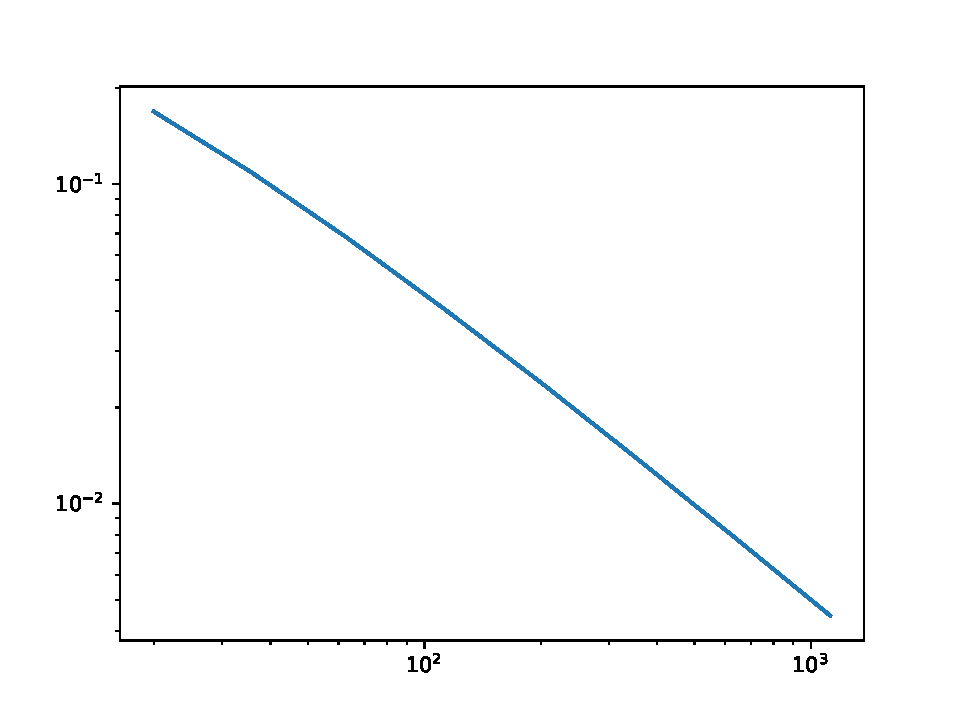
\includegraphics[width=0.75\textwidth]{code/advect_conv.pdf}
    \caption{\label{fig:advect_conv}}
\end{figure}

